\section{System Architecture and Implementation}
\label{sec:architecture}

The development of the Neural Processing Unit (NPU) followed a stringent top-down design methodology, spanning high-level software models, bit-accurate C verification, parameterized SystemVerilog Hardware Description Language (HDL), and comprehensive testbenches.

\subsection{Fundamental Hardware Challenges}
Mapping a neural network to a physical digital circuit introduces several distinct hardware challenges that dictate the architectural topology:
\begin{enumerate}
    \item \textbf{Memory Bandwidth and Size:} Fully connected networks require massive amounts of weights and biases to be stored and moved. Feeding thousands of parameters into the MAC units every cycle can easily saturate the memory bus bandwidth. 
    \item \textbf{Overflow and Quantization:} The core mathematical operation of a fully connected neural network is the linear combination of inputs and weights, generating large partial products.
    \begin{equation}
        u_j = \sum_{i=1}^{n} w_{ji} x_i + b_j
    \end{equation}
    Followed by a non-linear activation:
    \begin{equation}
        y_j = \text{ReLU}(u_j) = \max(0, u_j)
    \end{equation}
    Where $x_i$ represents the input activations, $w_{ji}$ the synaptic weights, $b_j$ the biases, and $y_j$ the final output. Preserving the correct values of these large partial products ($u_j$) without succumbing to integer overflow or utilizing complex saturation logic is a critical datapath obstacle.
\end{enumerate}

To overcome these challenges, we implemented a purely spatial datapath as illustrated in Fig. \ref{fig:nn_arch}, physically unrolling each layer rather than relying on a centralized memory pool.

\begin{figure}[ht]
    \centering
    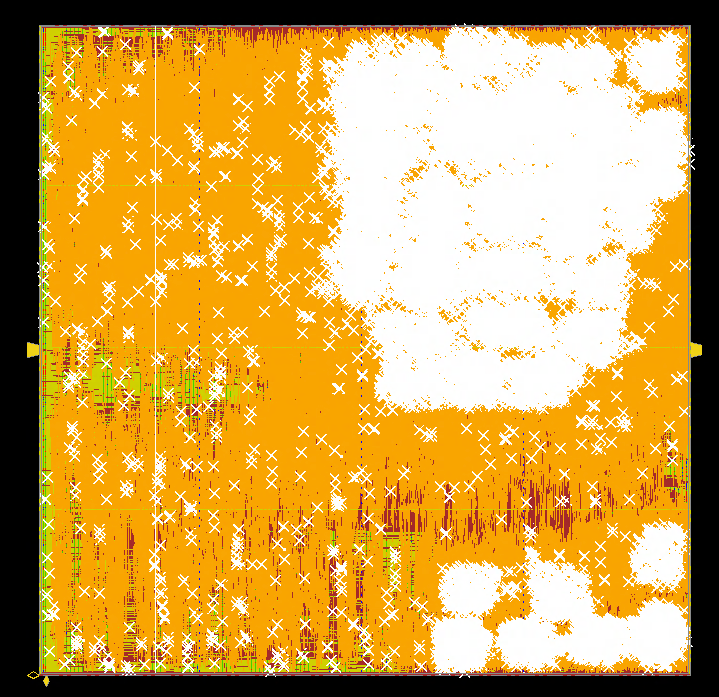
\includegraphics[width=\columnwidth]{Fig/nn_arch.png}
    \caption{Visual representation of the fully connected network topology. Our hardware unrolls these computational nodes across dedicated MAC lanes.}
    \label{fig:nn_arch}
\end{figure}

\subsection{Software Flow and Pre-processing (Python)}
The neural network was first defined and trained in a high-level software environment using PyTorch. The model was trained using a standard Adam optimizer and CrossEntropyLoss for 15 epochs on the MNIST dataset, achieving a baseline floating-point accuracy of approximately 97.5\%.

Following training, Python automation scripts (such as \texttt{gen\_npu\_weights.py}) were developed to bridge the gap between software and hardware. These scripts performed fixed-point quantization (translating floating-point tensors into 16-bit integer strings) and automatically dumped the biases and weights. To ensure ASIC synthesis compatibility, the scripts formatted the arrays directly into nested SystemVerilog \texttt{parameter} arrays within a custom \texttt{weight\_pkg.sv} rather than relying on dynamic \texttt{\$readmemh} operations, which standard synthesis tools often struggle to map efficiently to logical ROMs. 

\subsection{Bit-Accurate Verification Model (C Language)}
Before embarking on RTL design, a software-level golden model was implemented in C (\texttt{neural\_net.c}). This model perfectly mirrored the fixed-point constraints of the planned hardware.
\begin{itemize}
    \item \textbf{Quantization Verification:} It applied a strict 16-bit fractional format (e.g., Q12 format). 
    \item \textbf{Execution Validation:} The C application parsed the identical \texttt{.txt} hex arrays generated by Python and ran the inference algorithm sequentially. By comparing the C output to the PyTorch results, we validated that the quantization loss was acceptable and provided an ironclad reference for the hardware testbench.
\end{itemize}

\subsection{Hardware Architecture (SystemVerilog)}
The core NPU is implemented in SystemVerilog, emphasizing hardware elegance and efficiency.
\begin{itemize}
    \item \textbf{Network Topology:} The hardware computes a 4-layer fully connected architecture with layer sizes scaling as \texttt{784} $\to$ \texttt{32} $\to$ \texttt{16} $\to$ \texttt{16} $\to$ \texttt{10}. It is heavily parallelized, deploying 32 independent MAC (Multiply-Accumulate) lanes.
    \item \textbf{Activation Function:} Unlike traditional edge NPUs that utilize a Sigmoid activation (which requires expensive Look-Up Table (LUT) memory blocks to approximate the exponential calculation), our design employs the Rectified Linear Unit (ReLU). In RTL, ReLU is merely a zero-latency digital multiplexer (\texttt{in > 0 ? in : 0}), drastically reducing the area overhead and logic depth delay.
    \item \textbf{Datapath and Accumulation:} The input activations and weights are purely 16-bit. However, inside the processing elements, the data is pushed onto an expanded precision accumulator path (e.g., 64-bit bounds allowed by SystemVerilog parametrics: \texttt{[2*DATA\_WIDTH-1:0]}). This massive dynamic range organically prevents overflow, entirely eliminating the need for complex and slow saturating addition logic that plagued baseline models. This MAC unit structure is detailed in Fig. \ref{fig:mac_arch}.
    \item \textbf{Parameterization:} Through the use of \texttt{generate-for} loops and parameterized modules, the single \texttt{layer.sv} base module can dynamically instantiate routing neurons. This makes the SystemVerilog codebase highly scalable to deeper architectures without manual rewrites.
\end{itemize}

\begin{figure}[ht]
    \centering
    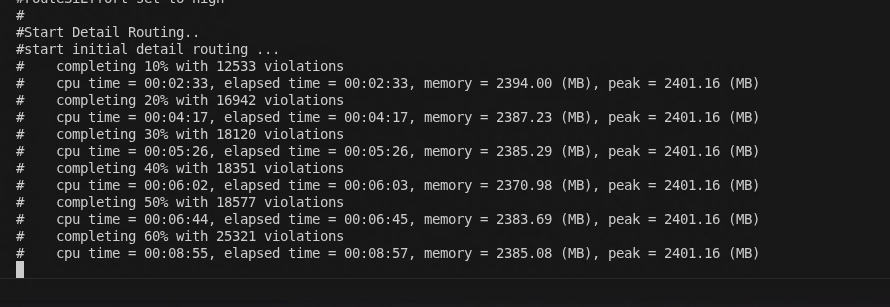
\includegraphics[width=0.85\columnwidth]{Fig/mac_arch.png}
    \caption{Single MAC Lane Architecture. The 16-bit inputs enter the multiplier, dropping into a 64-bit accumulator to naturally prevent saturation, followed by a zero-latency ReLU multiplexer.}
    \label{fig:mac_arch}
\end{figure}

\subsection{Testbench and Output Verification}
To verify the complex RTL datapath, an advanced verification environment was critical. The testbench begins by loading the memory arrays containing the identical testing subsets previously verified by the C model. 
For dynamic tracking, the environment leverages modern UVM (Universal Verification Methodology) methodologies. We developed systemic Coverage Hooks monitoring the internal \texttt{l0\_relu} through \texttt{l3\_relu} interfaces. A dedicated \texttt{cg\_layer\_activations} functional coverage model was explicitly queried, eventually achieving exactly 100.0\% Activation Coverage. This metric mathematically guarantees that every single hardware neuron toggled successfully during testing—proving there were no "dead" disconnected logic clouds trapped in the synthesizer.
